%%%%%%%%%%%%%%%%%%%%%%%%%%%%%%%%%%%%%%%%%%%%%%%%%%%%%%%%%%%%%%%%%%%%%
% LaTeX Template: Project Titlepage Modified (v 0.1) by rcx
%
% Original Source: http://www.howtotex.com
% Date: February 2014
% 
% This is a title page template which be used for articles & reports.
% 
% This is the modified version of the original Latex template from
% aforementioned website.
% 
%%%%%%%%%%%%%%%%%%%%%%%%%%%%%%%%%%%%%%%%%%%%%%%%%%%%%%%%%%%%%%%%%%%%%%

\documentclass[11pt]{report}
\usepackage[a4paper]{geometry}
\usepackage[myheadings]{fullpage}
\usepackage{fancyhdr}
\usepackage{lastpage}
\usepackage{graphicx, wrapfig, subcaption, setspace, booktabs}
\usepackage[T1]{fontenc}
\usepackage[font=small, labelfont=bf]{caption}
\usepackage{fourier}
\usepackage[protrusion=true, expansion=true]{microtype}
\usepackage[english]{babel}
\usepackage{sectsty}
\usepackage{url, lipsum}
\usepackage{amsmath}

\newcommand{\HRule}[1]{\rule{\linewidth}{#1}}
\onehalfspacing
\setcounter{tocdepth}{5}
\setcounter{secnumdepth}{5}

%-------------------------------------------------------------------------------
% HEADER & FOOTER
%-------------------------------------------------------------------------------
\pagestyle{fancy}
\fancyhf{}
\setlength\headheight{15pt}
\fancyhead[L]{Terrence Ho}
\fancyhead[R]{Experiment 5}
\fancyfoot[R]{Page \thepage\ of \pageref{LastPage}}
%-------------------------------------------------------------------------------
% TITLE PAGE
%-------------------------------------------------------------------------------

\begin{document}

\title{ \normalsize \textsc{Physics 4AL}
        \\ [2.0cm]
        \HRule{0.5pt} \\
        \LARGE \textbf{\uppercase{Experiment 5: Harmonic Oscillator Part I:
        Spring Oscillator}}
        \HRule{2pt} \\ [0.5cm]
        \vspace*{2\baselineskip}}

\date{}

\author{
        Terrence Ho | ID: 804793446 \\ 
        Date of Lab: May 16th, 2017 \\
        Lab Section: Tuesday, 5 P.M.\\
        T.A.: David Bauer\\
        Lab Partners: Robathan Harries \\
        Abstract: 165 words\\
        Report: 2189 words\\
    }
\maketitle
\tableofcontents
\newpage

%-------------------------------------------------------------------------------
% Section title formatting
\sectionfont{\scshape}
%-------------------------------------------------------------------------------

%-------------------------------------------------------------------------------
% BODY
%-------------------------------------------------------------------------------
\addcontentsline{toc}{section}{Abstract}
\begin{center}
\title{
    \Large \textbf{\uppercase{Investigating Resonant Frequency in Damped and Undamped Oscillations}}
}

T. Ho\footnote{Henry Samueli School of Engineering and Applied Science,
University of California, Los Angeles}
\end{center}

In Newtonian mechanics, a mass suspended on a spring will undergo harmonic
motion if acted by an outside force.
The objective of the experiment was to investigate the motion of damped and
undamped oscillations. Specifically, we wanted to find whether
resonant frequencies in both types of oscillations would be equivalent.
A mass was hung from a spring attached to a vertical force sensor, which 
measured both voltage and time. Magnets provided a damping force when passed
through a metal tube. Graphs of voltage vs time were plotted to
find the relationship between these values. Based on the resonant frequency 
of the undamped oscillation found
from our data, we calculated a value of the damped resonant frequency and
comapred it to the measured value of damped resonant frequency.  Through this, 
we confirmed the 
experimental resonant frequency matched calculated predicted values, which was
0.67 $\pm$ 0.02 Hz. We found that
the resonant frequency for undamped oscillations and damped oscillations (both
measured and calculated) are the exact same.  

\newpage
\begin{figure}[h!]
    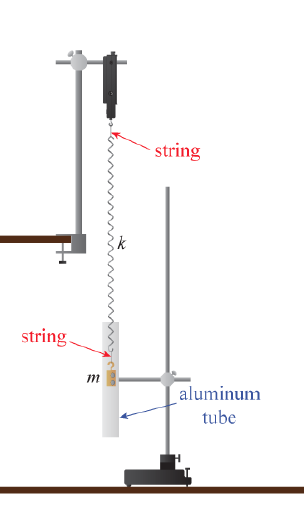
\includegraphics[]{setup.png}
    \captionsetup{labelformat=empty}
    \caption{\textbf{Figure 5.1 Setup for Oscillation Experiment.}  The sensor
    provides the readout of voltage during oscillation motion.  The weight has
    magnets that can provide a damping force if passed through the aluminum
    tube.  Be sure to decouple the spring from the mass and the force sensor to
    produce the most accurate data.  Figure
reproduced (with permission) from Fig. 5.1 by Campbell, W. C. et al.$^1$}
\addcontentsline{toc}{subsection}{Figure 5.1}
\end{figure}

\newpage
\section*{Introduction}
\addcontentsline{toc}{section}{Introduction}
Oscillations are caused by an acting force and a restoring force exerted by a
spring. If an object is oscillating and there is no other force acting on it, it
is in simple harmonic motion and has a constant amplitude and frequency.  This
frequency is also known as the resonant frequency, where it's amplitude will be
greatest.  

Damped oscialltions are oscillations that are affected by an outside force that
causes the amplitudes of its oscillation to decrease exponentially.  This is
known as the damping term.  Damping time is the time it takes for a damping
force to decay the amplitude by a factor of \(\frac{1}{e}\).  Damped
oscillations are affected by something called the Q-factor, which describes how
energy is lost in a resonant element which in our experiment is the mass and
spring.  These terms can all be used to find the resonant frequency of a damped
oscillation, which we will see later.  

In our experiment, we sought to observe both undamped and damped oscillations,
with the ultimate goal of finding the resonant frequency.  By hanging a mass
onto a force sensor and measuring voltage produced by the mass over time,
we were able to measure the resonant frequency produced by undamped and damped
oscillations, and compare these values.

\section*{Methods}
\addcontentsline{toc}{section}{Methods}


The first step of the experiment is to determine the spring constant of the
spring we will hang our masses from.  A series of masses were hung from the
spring and the distance from the mass to the floor was measured and plotted.
The slope of the best fit line gives our spring constant \(k\) (\textbf{Figure
5.2}). 

\textbf{Figure 5.1} shows the layout of our experiment. 
With the force sensor (measuring voltage) attached to the computer, set a high sample
rate for the sensor so the voltage data is accurate.  Attach a small string to the
bottom of the hook, then attach the mass to the string (this is done to avoid
uncertainty that occurs when the spring rotates and turns as it stretches and
compresses).  The mass should have magnets on it's side so an aluminnum tube can
be used for the damped oscillation trial and slow the mass.  A small vertical force was
given to the spring mass system and let to oscillate for 40 seconds, during
which voltage and time are recorded. Do this twice, once without damping and
once with damping through the aluminum tube.

Any data recorded should be transferred over to Excel for analysis.  Other data
important to collect would be an offset voltage(to account for the fact the
voltage data may not be centered at zero) and mass of the weight used.  

\section*{Analysis}
\addcontentsline{toc}{section}{Analysis}

\subsection*{Derivations}
\addcontentsline{toc}{subsection}{Derivations}
We mentioned terms such as damping term, resonant frequency, damping time, and
Q-factor before, now we shall see how these terms are related.

The equation \[m\ddot{x} = -kx - b\dot{x}\] is the differential equation that
represents damped motion.  One solution to this differential equation is \[x(t)
    = Ae^{iwt}\]  By substituting this into the first equation we get
    \[-w^2mAe^{iwt} = -kAe^{iwt} - iwbAe^{iwt}\] which can simplify to \[mw^2 =
        k + iwb\] By solving this quadratic equation, we find that \[w =
    \frac{ib}{2m} \pm \sqrt{\frac{k}{m} - \frac{b^2}{4m^2}}\]  If we
    substitute what we just found into the solution to the differential equation
    stated previously, we find that \[x(t) = Ae^{i\bigg( \frac{ib}{2m} +
        \sqrt{\frac{k}{m} - \frac{b^2}{4m^2}}  \bigg)t}\] \[x(t) =
    Ae^{i\sqrt{\frac{k}{m} - \frac{b^2}{4m^2}}t} \times e^{-bt}{2m}\]
As stated previously, damping time $\tau$ is defined to be the time is takes for
a damped oscillation to decay by a factor of \(\frac{1}{e}\).  Damping time is
usually defined as \[\tau = \frac{2m}{b}\]
The frequency of damped oscillations can be found by dividing the angular
frequency by 2$\pi$, or \[f_{damped} = \frac{w_{damped}}{2\pi} \equiv
    \frac{1}{2\pi}\sqrt{\frac{k}{m} - \frac{b^2}{4m^2}} = f_0\sqrt{1 -
    \frac{b^2}{4m^2}}\]  By definition, we also know that \[f_{damped} \equiv
f_0\sqrt{1 - \frac{1}{4Q^2}}\]  By setting these two equations equal to one
another, we find \[ \sqrt{1 - \frac{1}{4Q^2}} = \sqrt{1 - \frac{b^2}{4km}}\]
We solve and simpilfy for Q to get \[Q = \frac{\sqrt{km}}{b}\] 
Thus, Q can be found if we know the mass, the spring constant, and the damping
term.  We can find the damping term \(b\) by first knowing the damping time
$\tau$ and dividing twice the mass by \(b\).

\subsection*{Plots and Graphs}
\addcontentsline{toc}{subsection}{Plots and Graphs}

We first determined the spring constant of the spring by hanging masses of 0 g, 50 g,
100 g, 150 g, and 200 g, and plotting these masses against the distance
remaining from the ground to the spring when placed onto the spring (the
uncertainty of the masses was 0.0005 kg, half the lowest precision of our scale).  This is
illustrated in \textbf{Figure 5.2}.  The spring constant is determined to be
3.2 $\pm$ 0.2 N/m.

The mass \(m\) on the spring we used for our experiment was 175 $\pm$ 0.5 g.  

To predict our resonant frequency, we used the equation \(f_0 =
\frac{1}{2\pi}\sqrt{\frac{k}{m}}\), where \(k\) is the spring constant found on
\textbf{Figure 5.2} and \(m\) is the mass of the weight on spring.  Using the
propagation of uncertainty, \(\frac{\delta f_0}{f_{0, best}} =
\sqrt{\bigg(\frac{\delta k}{2k} \bigg)^2 + \bigg(\frac{\delta m}{2m} \bigg)^2}
\), to find the uncertainty for \(f_0\), we find that \(f_{0, predict} = 0.67
\pm 0.02\) Hz. 



\begin{figure}
    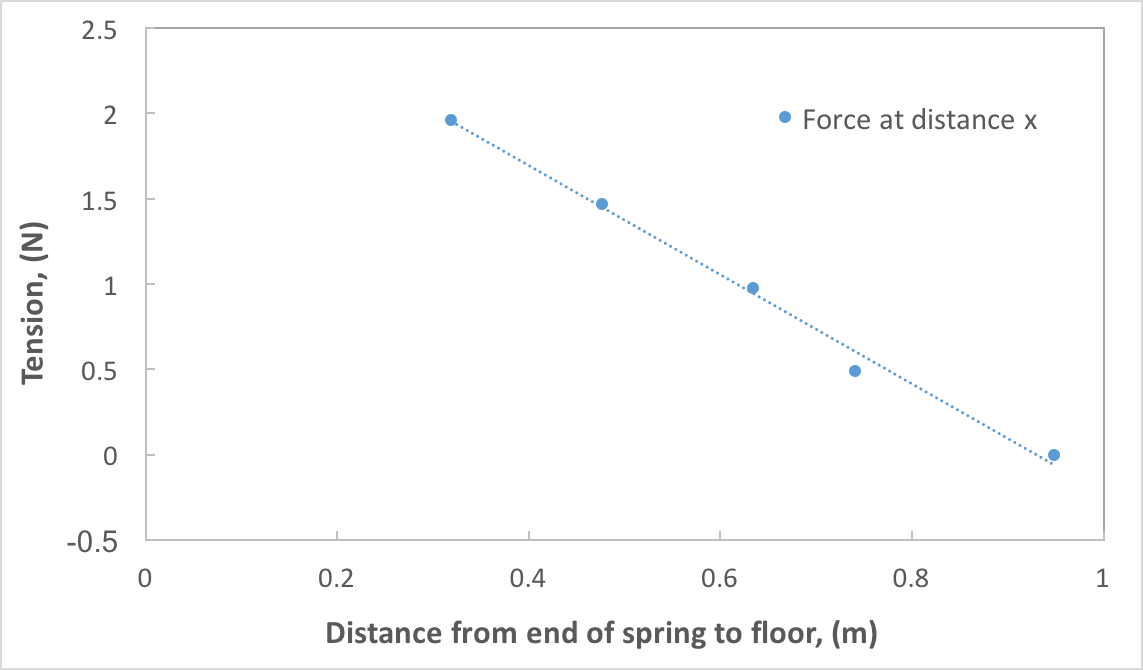
\includegraphics[width=\linewidth]{ForceDistance.png}
    \captionsetup{labelformat=empty}
    \caption{\textbf{Figure 5.2 Measuring Spring Constant of a Spring.}  Masses
    used were 0 g, 50 g, 100 g, 150 g, and 200 g.  The best fit line has the
    equation \(F = (-3.2 \pm 0.2)x + (2.9 \pm 0.1)\) The spring constant was found to be \(3.2 \pm
0.2\) N/m.}
\addcontentsline{toc}{subsection}{Figure 5.2}
\end{figure}

\begin{figure}
    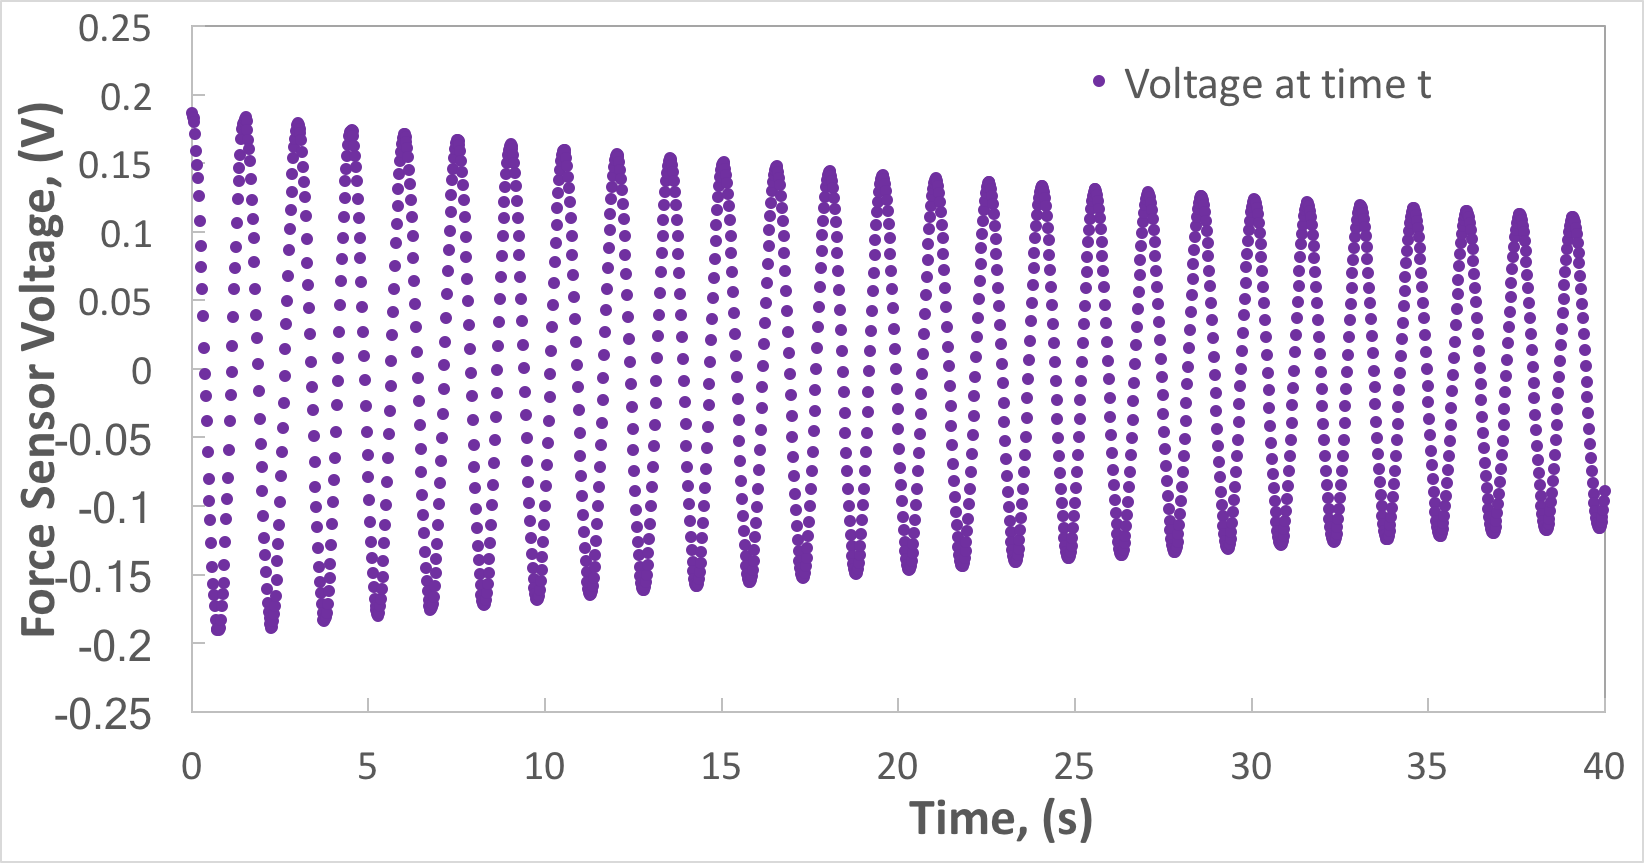
\includegraphics[width=\linewidth]{VoltageTime1.png}
    \captionsetup{labelformat=empty}
    \caption{\textbf{Figure 5.3 Simple Harmonic Motion of Spring.} The x-axis
    shows time of reading and the y-axis shows the voltage measured by the force
sensor at that time. An offset of 0.0327 V was added to each voltage to center
our readings at V = 0. The \(f_0\) found from this figure is 0.661 $\pm$ 0.002 Hz.}
\addcontentsline{toc}{subsection}{Figure 5.3}
\end{figure}

In both \textbf{Figure 5.3} and \textbf{Figure 5.4}, we plotted our measured
voltage values at each time. The data is presented with
an offset to the voltage, which accounts for the fact the equilibrium voltage
was not 0 V and to avoid drifting in our data for the damping oscillation in
\textbf{Figure 5.4}.  The offset value is 0.0327 V.

\textbf{Figure 5.3} shows our plotted values of voltage \(V\) at time \(t\) for
the undamped oscillation. We derived our experimental value of $f_{0, undamped}$ by taking the
maxima at several different points, zooming in and finding the maximum value and
time of each peak.  The undamped resonant frequency $f_{0}$ is then equal to \(\frac{n -
1}{t_n - t_1}\), where \(n\) is the peak number and \(t\) is the time when that
peak occured. We took several trials of this data to find an uncertainty range
(standard deviation of the data divided by the number of trials),
and the resulting frequency was \(f_{0} = 0.661 \pm 0.002\) Hz.  

Similarly, we plotted the measured voltage values at each time for the damped
oscillation in \textbf{Figure 5.4}. We derived our experimental value of
$f_{damped}$ by taking the
maxima at several different points, zooming in and finding the maximum value and
time of each peak.  The damped resonant frequency is then equal to \(\frac{n -
1}{t_n - t_1}\), where \(n\) is the peak number and \(t\) is the time when that
peak occured. We took several trials of this data to find an uncertainty range
(standard deviation of the data divided by the number of trials),
and the resulting frequency was \(f_{damped} = 0.660 \pm 0.003\) Hz.  

We can see that in both the damped and undamped oscillations, the resonant
frequencies \(f_0\) and \(f_{damped}\) calculated from our experiment were within the uncertainty
range of our predicted resonant frequency \(f_{0, predict}\), which was 0.67
$\pm$ 0.02 Hz.  Thus our calculated values are accurate relative to our
predicted value and resonant frequencies in undamped and damped oscillations are
the same.



\begin{figure}
    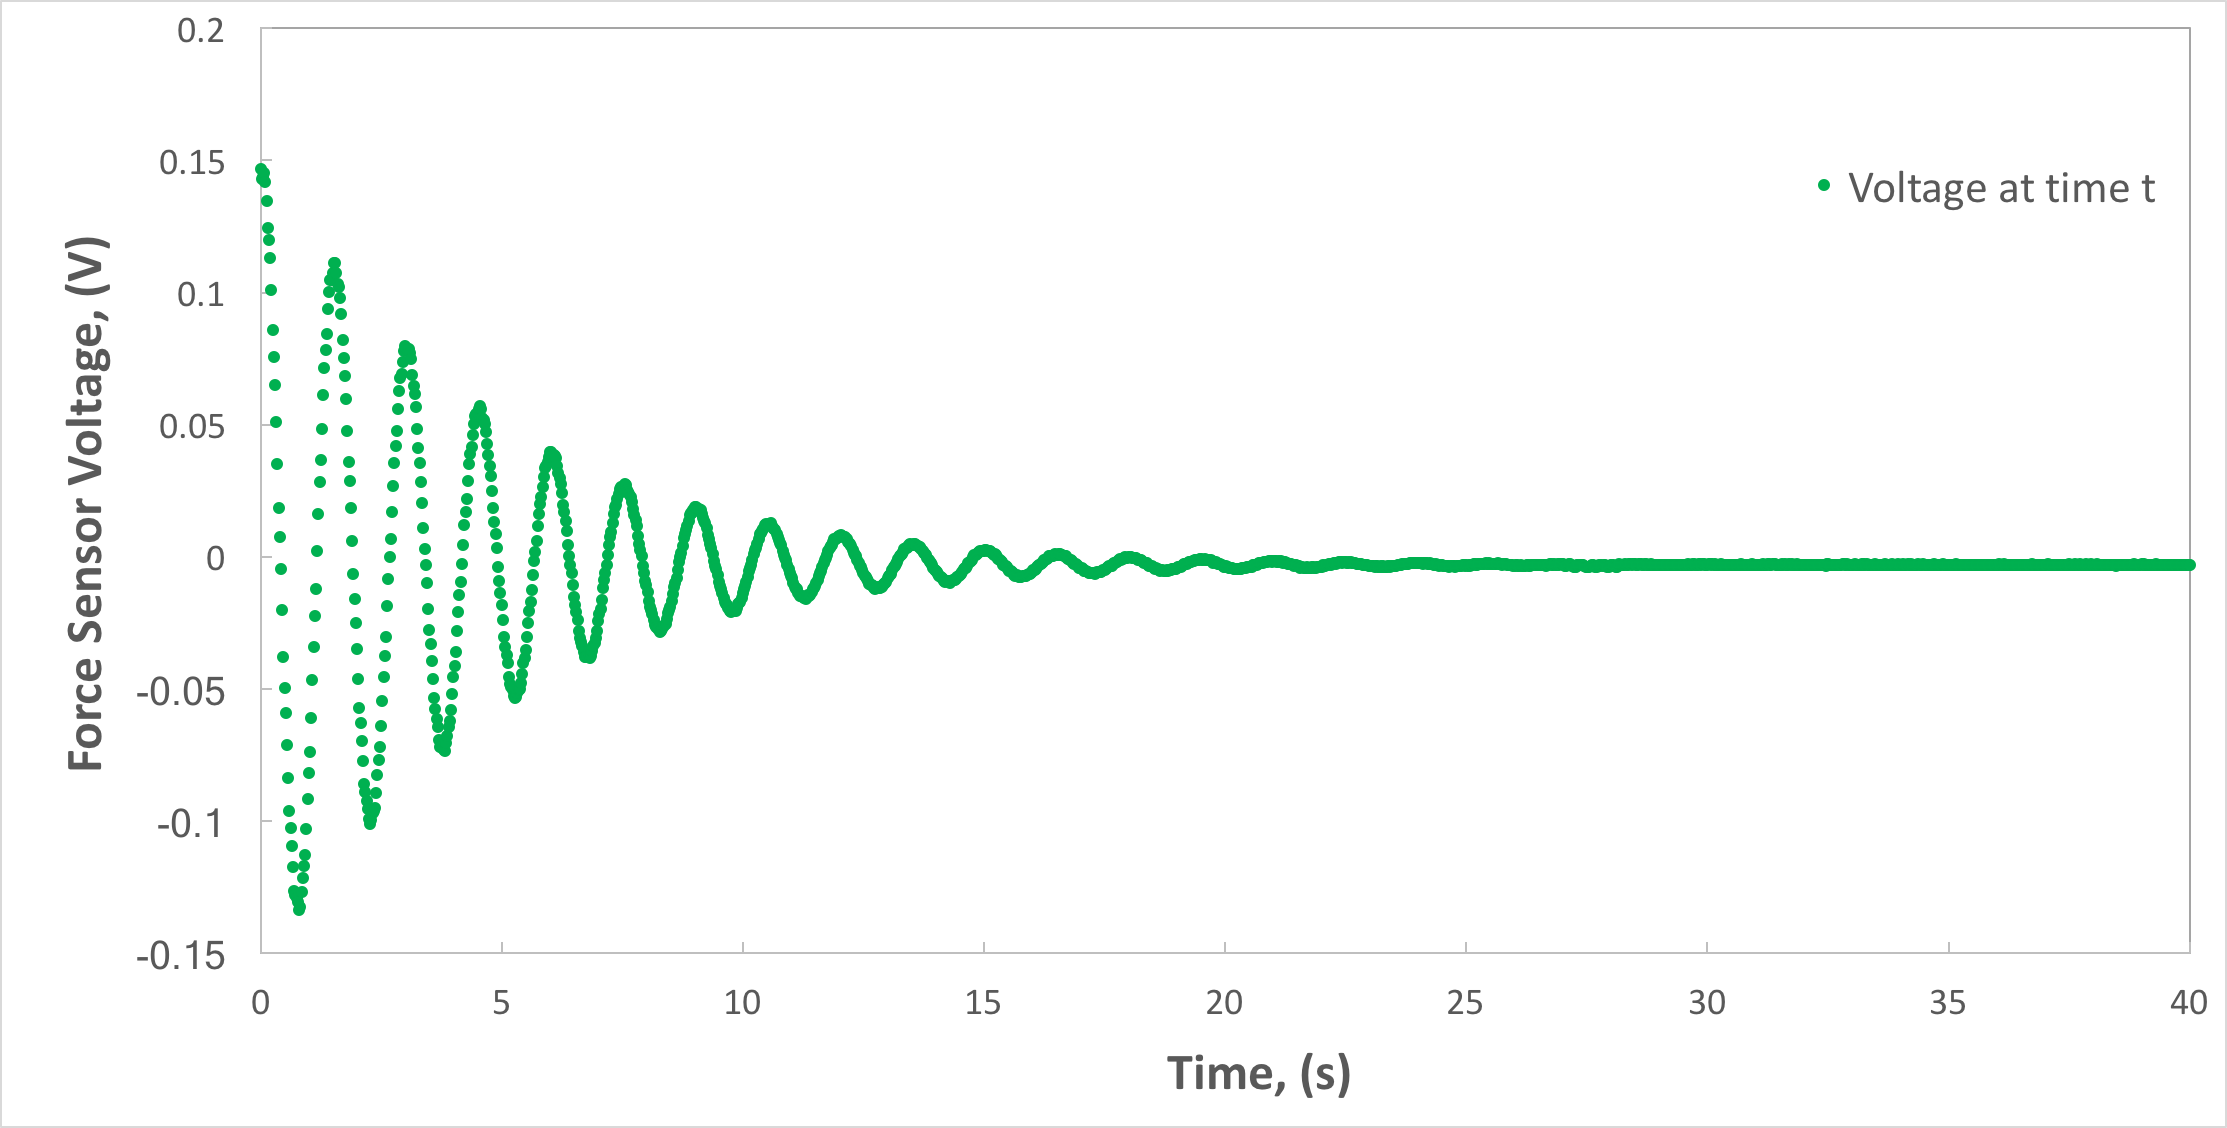
\includegraphics[width=\linewidth]{VoltageTime2.png}
    \captionsetup{labelformat=empty}
    \caption{\textbf{Figure 5.4 Damped Oscillation of a Spring.}  The x-axis
    shows the time of reading and the y-axis shows the voltage measured by the
force sensor at that time.  The offset was 0.0327 V, which was added to each
voltage value to center our readings. The \(f_0\) value derived from this graph
is 0.660 $\pm$ 0.003 Hz.}
\addcontentsline{toc}{subsection}{Figure 5.4}
\end{figure}

We can also determine damping time from \textbf{Figure 5.4}.  Damping time is the time for
the damped osciallation's amplitude to decrease by \(\frac{1}{e}\), which will
only decay exponentially if damping is caused by a velocity-dependent force, and
not by a friction force.  After ensuring our voltage-time plot in \textbf{Figure
5.4} is centered around V = 0, we took the peak voltages for several extrenum,
and calculated the ratio of peak voltages from one peak to the next.  The ratio
between amplitudes was plotted in \textbf{Figure 5.5}, which we can see ranges
from 0.81 to 0.86.  The ratio values shown in \textbf{Figure 5.5} do not 
indicate any upward or downward trend, which means we have chosen a correct
value for the voltage offset.  By setting a correct offset value, we have
avoided a drift in our voltage data and now our future measurements not be
affected by the fact that the equilibrium voltage was not centered at 0 V.


\begin{figure}
    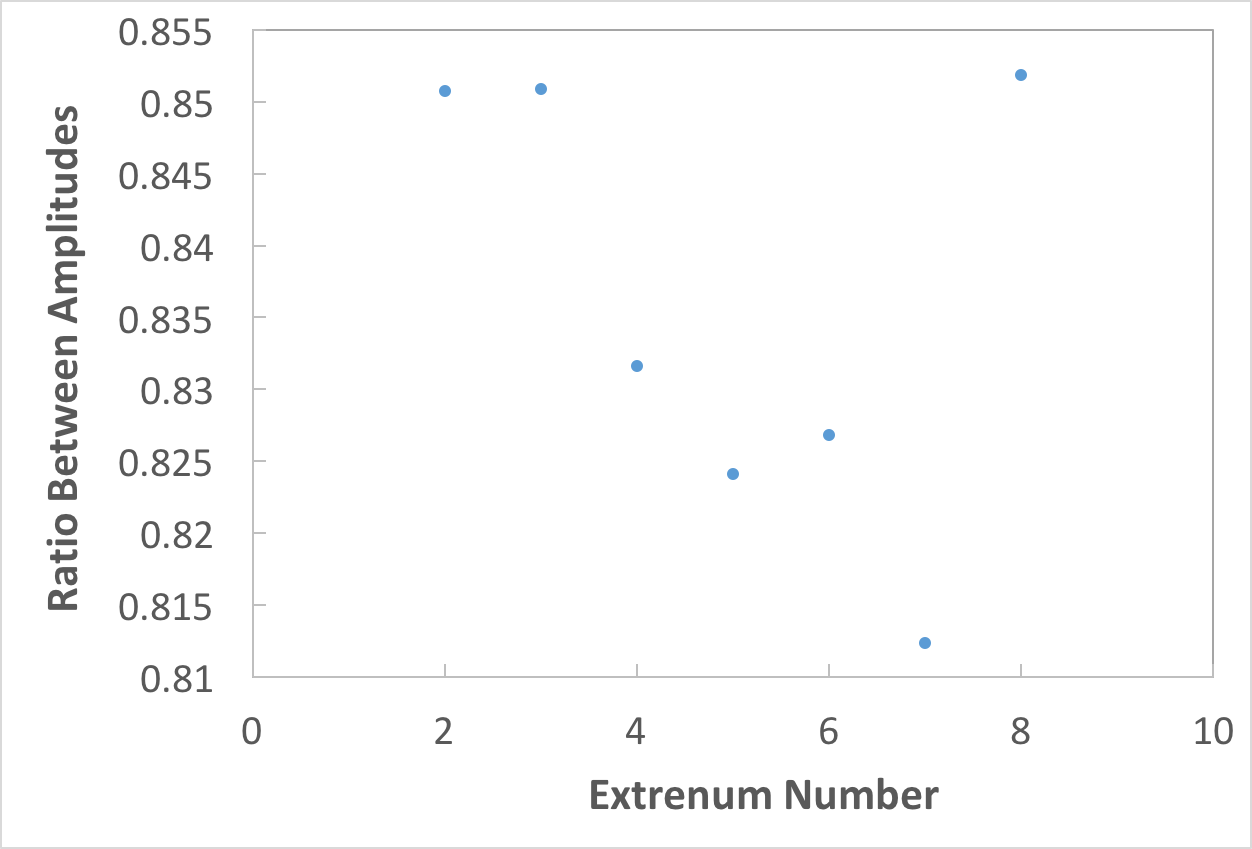
\includegraphics[width=\linewidth]{Extrenum.png}
    \captionsetup{labelformat=empty}
    \caption{\textbf{Figure 5.5 Ratios of Peak Amplitudes} Graph of ratios of
    voltages from peaks of damped oscillations.  Ratios range from 0.81 to 0.86.}
    \addcontentsline{toc}{subsection}{Figure 5.5}
\end{figure}

Each ratio measurement was converted to damping time $\tau$ with this equation:
\(\tau = -\Bigg(\frac{T}{ln\bigg(\frac{V(t + T)}{V(t)}\bigg)}\Bigg)\).  We
collected each damping time calculated for each ratio and averaged them to find
the mean damping time, which was $\tau$ = 8.5 $\pm$ 0.3 s (uncertainties found by taking
the standard deviation divided by number of ratios).  

We can determine damping term \(b\) by dividing twice the mass by the mean
damping time, or \(b = \frac{2 * m}{\tau}\).  With a mass of 0.175 kg and using
the previously found mean damping time, we find that \(b = 0.04 \pm 0.03\) kg/s
(uncertainties found by propagation of uncertainties).  

Next, we can also determine something called the Q-factor from our damped
oscillation, which indicates energy loss in a resonant element which in this
experiment is the spring-mass system.  The equation for Q is 
\(Q = \frac{\sqrt{k * m}}{b}\), so we can
substitute our previously found value for \(b\), as well as the spring constant
\(k\) and mass \(m\) to find \(Q\).  By doing this, we calculate that \(Q =
18.2 \pm 0.8\).  

Lastly, we can use the Q factor to see if our calculated value for
\(f_{damped}\) matches the one we measured by sampling extrenum of
\textbf{Figure 5.4}.  Using the equation \(f_{damped} = f_0 * \sqrt{1 -
\frac{1}{4Q^2}}\), where \(f_0\) is the resonant frequency found by sampling
peaks in \textbf{Figure 5.3} and Q is the Q-factor found previously.  We
calculate that \(f_{damped} = 0.66 \pm 0.04\) Hz.  We find the measuring and
calculating the value of \(f_{damped}\) results in the exact same values, as our
measured value of \(f_{damped}\) falls within the uncertainty range of the
\(f_{damped}\) value we just calculated.

As a bonus, we tried to find the resonant frequency by doing a Fast Fourier
Transformation(FFT) on our damped oscillation data. By taking the width of the
peak at \(\frac{1}{\sqrt{2}}\) of the height of the maximum value, we can
determine the width of the change of resonance \(\Delta f\).  The FFT's peak was
0.025 Hz wide.  Because Q is large, Q can be found as the ratio of resonance
frequency to resonance width, or \(Q = \frac{f_0}{\Delta f}\). The base of the
FFT determines the resonant frequency of the oscillations, which was at 0.6468
Hz.  Using the previously defined formula, \(Q = 25.872\).  
The value of Q calculated from our FFT is higher by 7.7 than the value of Q
derived from our calculations of the damped oscillation. 

\section*{Conclusion}
\addcontentsline{toc}{section}{Conclusion}
We performed our experiment to study simple harmonic motion and damped
oscillations.  We wanted to verify if resonant frequency in both damped and
undamped oscialltions would be the same.  
Our predicted value of the resonant frequency was 0.67 $\pm$ 0.02 Hz.  
The resonant frequency from the undamped oscillation was 0.661 $\pm$ 0.002.  Our
measured value of \(f_{damped}\) from \textbf{Figure 5.4} was 0.660 $\pm$ 0.003
Hz.  The calculated value of \(f_{damped}\) was 0.66 $\pm$ 0.04 Hz.  All values of
the resonant frequency from both undamped and damped oscillations fell inside
the uncertainty range of the predicted \(f_0\).  We verified that the measured
and caluclated value of \(f_{damped}\) were the same.  Our experiment verifies
that the resonant frequency was the same regardless of damping and that multiple
ways of calculating the resonant frequency results in the same \(f_0\).

We note that although the our values of \(f_0\) fell within our predicted
frequency's uncertainty range our experimental values were lower than the
predicted value.  As such, we can attribute some external factors such as
friction to a loss of energy that makes our experimental values slightly lower
than the predicted value, which could slow the oscillations and lower the
frequency.  Another source of error could stem from the uncertainty value
of our spring constant was to the first decimal place, which gives a wide range
of possible error.  This wide range could have attributed to the slightly lesser
experimental values of \(f_0\) if the spring constant was actually lower than
\(k_{best}\) for our experimental trials.  This is a source of systematic error
that could be avoided by measuring the spring constant to a higher degree of
precision.


\newpage
\section*{References}
\addcontentsline{toc}{section}{References}
\begin{enumerate}
    \item Campbell, W. C. et al. Physics 4AL: Mechanics Lab Manual (ver. April
        3, 2017). (Univ. California Los Angeles, Los Angeles, California).
\end{enumerate}




\end{document}



%-------------------------------------------------------------------------------
% REFERENCES
%-------------------------------------------------------------------------------
% \newpage
% \section*{References}
% \addcontentsline{toc}{section}{References}

% Anand, U., 2010. The Elusive Free Radicals, \textit{The Clinical Chemist,} [e-journal] Available at:<\url{http://www.clinchem.org/content/56/10/1649.full.pdf}> [Accessed 2 November 2013]
% \newline
% \newline

% Biology Forums, 2012. \textit{Normal glomerulus. Acute glomerulonephritis.} [online] Available at: <\url{http://biology-forums.com/index.php?action=gallery;sa=view;id=9284}> [Accessed 23 October 2013].
% \newline
% \newline

% Budisavljevic, M., Hodge, L., Barber, K., Fulmer, J., Durazo-Arvizu, R., Self, S., Kuhlmann, M., Raymond, J. and Greene, E., 2003. Oxidative stress in the pathogenesis of experimental mesangial proliferative glomerulonephritis, \textit{American Journal of Physiology - Renal Physiology,} 285(6), pp. 1138-1148.
% \newline
% \newline

% Chien, C., Lee, P., Chen, C., Ma, M., Lai, M. and Hsu, S., 2001. De Novo Demonstration and Co-localization of Free-Radical Production and Apoptosis Formation in Rat Kidney Subjected to Ischemia/Reperfusion, \textit{Journal of the American Society of Nephrology,} 12(5), pp. 973-982.
% \newline
% \newline

% Couser, W., 1993. Pathogenesis of glomerulonephritis, \textit{Kidney International Supplements,} 42, pp. 19-26.
% \newline
% \newline

% De Gasparo, M., 2002. Angiotensin II and nitric oxide interaction, \textit{Heart Failure Reviews,} [e-journal] Available at:<\url{http://www.ncbi.nlm.nih.gov/pubmed/12379820}> [Accessed 26 October 2013]
% \newline
% \newline

% Edinburgh Renal Education Pages, 2012. \textit{Glomerulonephritis} [online] Available at: <\url{http://www.edrep.org/pages/textbook/glomerulonephritis.php}> [Accessed 25 October 2013].
% \newline
% \newline

% Forbes, J., Coughlan, M. and Cooper, M., 2008. Oxidative Stress as a Major Culprit in Kidney Disease in Diabetes, \textit{Diabetes,} 57(6), pp. 1446-1454.
% \newline
% \newline

% Geeky Medics, 2010. \textit{Glomerulonephritis} [online] Available at: <\url{http://geekymedics.com/2010/10/27/glomerulonephritis/}> [Accessed 25 October 2013].
% \newline
% \newline

% Gryglewski, R., Palmer, R., Moncada, S., 1986. Superoxide anion is involved in the break­down of endothelium derived relaxing factor, \textit{Nature,} 320, pp. 454-456.
% \newline
% \newline

% Halliwell, B., 2001. Free Radicals and other reactive species in Disease, \textit{Encyclopedia of Life Sciences,} [e-journal] Available at:<\url{http://web.sls.hw.ac.uk/teaching/level4/bcm1_2/reading/oxidative_stress/files/Oxidative_stress.pdf}> [Accessed 19 October 2013]
% \newline
% \newline

% Huang, H., Patel, P. and Salahudeen, A., 2001. Lazaroid compounds prevent early but not late stages of oxidant-induced cell injury: potential explanation for the lack of efficacy of lazaroids in clinical trials, \textit{Pharmacological Research,} 41(1), pp. 55-61.
% \newline
% \newline

% Klinger, J., Abman, S. and Gladwin, M., 2013. Nitric Oxide Deficiency and Endothelial Dysfunction in Pulmonary Arterial Hypertension, \textit{American Journal of Respiratory and Critical Care Medicine,} 188(6), pp. 639-646.
% \newline
% \newline

% Lindemann, I., Boettcher, J., Oertel, K., Pasternack, R., Heine, A. and Klebe, G. 2012. Inhibitors of Transglutaminase 2: A therapeutic option in celiac disease, \textit{To be Published,} [e-journal + PDB structure] Available at:<\url{http://www.ebi.ac.uk/pdbe-srv/view/entry/3s3s/summary}> [Accessed 24 October 2013]
% \newline
% \newline

% Mayo Clinic, 2011. \textit{Glomerulonephritis} [online] Available at: <\url{http://www.mayoclinic.com/health/glomerulonephritis/DS00503/}> [Accessed 20 October 2013].
% \newline
% \newline

% McCord, J., Roy, R. and Schaffer, S., 1985. Free radicals and myocardial ischemia. The role of xanthine oxidase, \textit{Advances in myocardiology,} [e-journal] Available at:<\url{http://www.ncbi.nlm.nih.gov/pubmed/2982206}> [Accessed 24 October 2013]
% \newline
% \newline

% National Health Service, 2012. \textit{Causes of glomerulonephritis} [online] Available at: <\url{http://www.nhs.uk/Conditions/Glomerulonephritis/Pages/Causes.aspx}> [Accessed 20 October 2013].
% \newline
% \newline

% Niaudet, P., 2013. \textit{Overview of the pathogenesis and causes of glomerulonephritis in children.} [online] Available at: <\url{http://www.uptodate.com/contents/overview-of- \ the-pathogenesis-and-causes-of-glomerulonephritis-in-children}> [Accessed 21 October 2013].
% \newline
% \newline

% Ronco, P., 2013. \textit{Mechanisms of glomerular crescent formation.} [online] Available at: <\url{http://www.uptodate.com/contents/mechanisms-of-glomerular-crescent-formation}> [Accessed 21 October 2013].
% \newline
% \newline

% Rutchik, J., 2013. \textit{Toxic Neuropathy Clinical Presentation.} [online] Available at: <\url{http://emedicine.medscape.com/article/1175276-clinical#a0216}> [Accessed 26 October 2013].
% \newline
% \newline

% R\&D Systems, 2013. \textit{Technical Information. Ischemia/Reperfusion Injury.} [online] Available at: <\url{http://www.rndsystems.com/cb_detail_objectname_SP96_Ischemia.aspx}> [Accessed 28 October 2013].
% \newline
% \newline

% Salahudeen, A., 1999. Free Radicals in Kidney Disease and Transplantation, \textit{Saudi Journal of Kidney Diseases and Transplantation,} 10(2), pp. 137-143.
% \newline
% \newline

% Sarma, A., Mallick, A. and Ghosh, A., 2010. Free Radicals and Their Role in Different Clinical Conditions: An Overview, \textit{International Journal of Pharma Sciences and Research,} 1(3), pp. 182-192.
% \newline
% \newline

% Shah, S., Baliga, R., Rajapurkar, M. and Fonseca, V., 2007. Oxidants in Chronic Kidney Disease, \textit{Journal of the American Society of Nephrology,} 18(1), pp. 16-28.
% \newline
% \newline

% The University of Utah, Unknown. \textit{Glomerulonephritis} [online] Available at: <\url{http://library.med.utah.edu/WebPath/RENAHTML/RENALIDX.html#8}> [Accessed 25 October 2013].
% \newline
% \newline

% Wang, C. and Salahudeen, A., 1994. Cyclosporine nephrotoxicity: attenuation by an antioxidant -inhibitor of lipid peroxidation in-vitro and in-vivo, \textit{Transplantation,} 58, pp. 940-946.
% \newline
% \newline

% Wang, C. and Salahudeen, A., 1995. Lipid peroxidation accompanies cyclosporine nephrotoxicity: effects of vitamin E, \textit{Kidney International,} 47, pp. 927-934.
% \newline
% \newline

% Weiss, S., 1989. Tissue Destruction by Neutrophils, \textit{New England Journal of Medicine,} 320, pp. 365-376.
% \newline
% \newline



%-------------------------------------------------------------------------------
% SNIPPETS
%-------------------------------------------------------------------------------

%\begin{figure}[!ht]
%    \centering
%    \includegraphics[width=0.8\textwidth]{file_name}
%    \caption{}
%    \centering
%    \label{label:file_name}
%\end{figure}

%\begin{figure}[!ht]
%    \centering
%    \includegraphics[width=0.8\textwidth]{graph}
%    \caption{Blood pressure ranges and associated level of hypertension (American Heart Association, 2013).}
%    \centering
%    \label{label:graph}
%\end{figure}

%\begin{wrapfigure}{r}{0.30\textwidth}
%    \vspace{-40pt}
%    \begin{center}
%        \includegraphics[width=0.29\textwidth]{file_name}
%    \end{center}
%    \vspace{-20pt}
%    \caption{}
%    \label{label:file_name}
%\end{wrapfigure}

%\begin{wrapfigure}{r}{0.45\textwidth}
%    \begin{center}
%        \includegraphics[width=0.29\textwidth]{manometer}
%    \end{center}
%    \caption{Aneroid sphygmomanometer with stethoscope (Medicalexpo, 2012).}
%    \label{label:manometer}
%\end{wrapfigure}

%\begin{table}[!ht]\footnotesize
%    \centering
%    \begin{tabular}{cccccc}
%    \toprule
%    \multicolumn{2}{c} {Pearson's correlation test} & \multicolumn{4}{c} {Independent t-test} \\
%    \midrule    
%    \multicolumn{2}{c} {Gender} & \multicolumn{2}{c} {Activity level} & \multicolumn{2}{c} {Gender} \\
%    \midrule
%    Males & Females & 1st level & 6th level & Males & Females \\
%    \midrule
%    \multicolumn{2}{c} {BMI vs. SP} & \multicolumn{2}{c} {Systolic pressure} & \multicolumn{2}{c} {Systolic Pressure} \\
%    \multicolumn{2}{c} {BMI vs. DP} & \multicolumn{2}{c} {Diastolic pressure} & \multicolumn{2}{c} {Diastolic pressure} \\
%    \multicolumn{2}{c} {BMI vs. MAP} & \multicolumn{2}{c} {MAP} & \multicolumn{2}{c} {MAP} \\
%    \multicolumn{2}{c} {W:H ratio vs. SP} & \multicolumn{2}{c} {BMI} & \multicolumn{2}{c} {BMI} \\
%    \multicolumn{2}{c} {W:H ratio vs. DP} & \multicolumn{2}{c} {W:H ratio} & \multicolumn{2}{c} {W:H ratio} \\
%    \multicolumn{2}{c} {W:H ratio vs. MAP} & \multicolumn{2}{c} {\% Body fat} & \multicolumn{2}{c} {\% Body fat} \\
%    \multicolumn{2}{c} {} & \multicolumn{2}{c} {Height} & \multicolumn{2}{c} {Height} \\
%    \multicolumn{2}{c} {} & \multicolumn{2}{c} {Weight} & \multicolumn{2}{c} {Weight} \\
%    \multicolumn{2}{c} {} & \multicolumn{2}{c} {Heart rate} & \multicolumn{2}{c} {Heart rate} \\
%    \bottomrule
%    \end{tabular}
%    \caption{Parameters that were analysed and related statistical test performed for current study. BMI - body mass index; SP - systolic pressure; DP - diastolic pressure; MAP - mean arterial pressure; W:H ratio - waist to hip ratio.}
%    \label{label:tests}
%\end{table}
